\documentclass{article}
\usepackage{tikz}
\usepackage{pgfplots}
\pgfplotsset{width=7cm,compat=1.8}
\usepackage{pgfplotstable}
\usepackage{adjustbox}
\usepackage{diagbox}
\usepackage{colortbl}
\definecolor{LightRed}{RGB}{252,160,140}
\definecolor{LightBlue}{RGB}{140,186,252}
\newcolumntype{a}{>{\columncolor{LightRed}}c}
\usetikzlibrary{decorations.pathreplacing,calligraphy}

\begin{document}


%\diagbox[width=0.6 \textwidth/2, height=1cm]{Disciplinas}{Fases} & Inicio
%Elaboraci\'on & Construcci\'on & Transici\'on
    
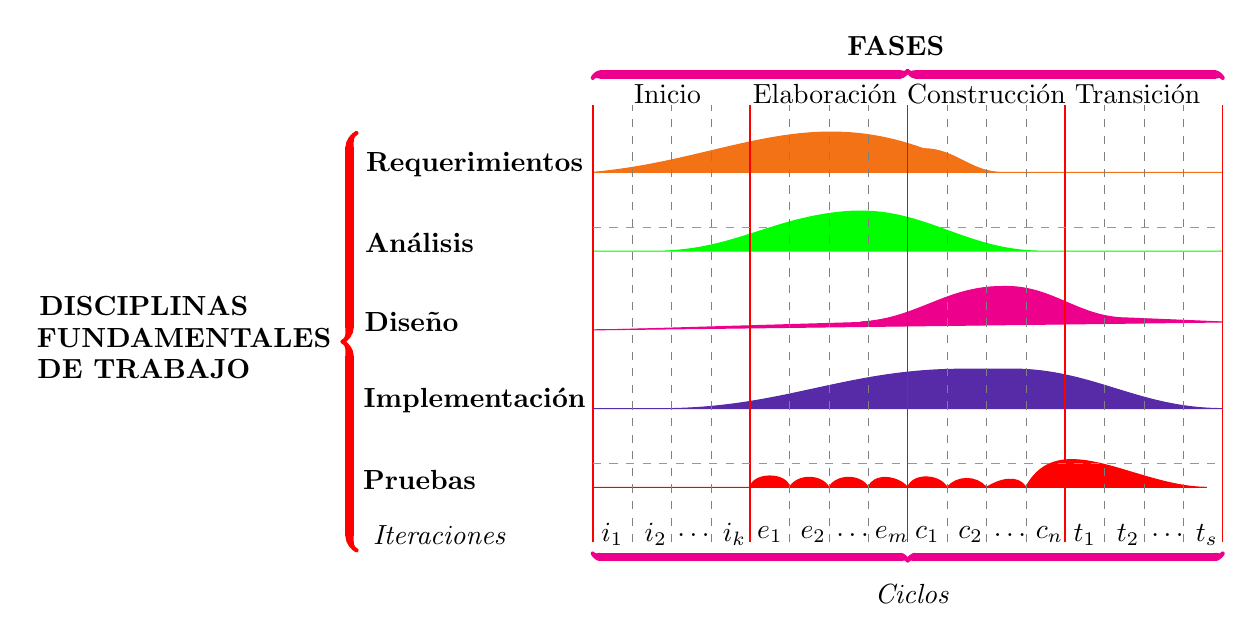
\begin{tikzpicture} 
\node (f0) at (8.65,0.6) {\bf FASES};
\draw [pen colour={magenta},decorate,decoration = {calligraphic brace},line width=3pt] (4.8,0.2) --  (12.8,0.2);
\node[] (f1) at (5.75,0) {Inicio}; 
\node (f2) at (7.75,0) {Elaboraci\'on};
\node (f3) at (9.8,0) {Construcci\'on};
\node (f4) at (11.72,0) {Transici\'on};

\node (d1) at (-0.9,-2.7) {\bf DISCIPLINAS};
\node (d2) at (-0.39,-3.1) {\bf FUNDAMENTALES}; 
\node (d3) at (-0.9,-3.5) {\bf DE TRABAJO};
\draw [pen colour={red},decorate,decoration = {calligraphic brace,amplitude=5pt},line width=3pt] (1.8,-5.8) -- (1.8,-0.5);

\node (d1) at (3.3,-0.9) {\bf Requerimientos};
\draw[fill,color=yellow!40!red] (4.8,-1) to[out=5,in=160] (9,-0.7) to[out=0,in=180] (10,-1) to (12.8,-1) to (4.8,-1);
\node (d2) at (2.6,-1.9) {\bf Análisis};
\draw[fill,color=green!150!yellow] (5.7,-2) to[out=2, in=185] (8,-1.5) to[out=5,in=180] (10.5,-2) to (12.8,-2) to (4.8,-2);
\node (d3) at (2.5,-2.9) {\bf Dise\~no};
\draw[fill,color=magenta!100!yellow] (8.2,-2.9) to[out=3,in=180] (10,-2.45) to[out=2,in=180] (11.6,-2.85) to (12.8,-2.9) to (4.8,-3);
\node (d4) at (3.3,-3.9) {\bf Implementaci\'on};
\draw[fill,color=orange!34!blue] (5.8,-4) to[out=1, in=180] (9.5,-3.5) to[out=1,in=180] (10,-3.5) to[out=2,in=180] (12.8,-4) to (4.8,-4);
\node (d5) at (2.6,-4.9) {\bf Pruebas};
\draw[fill,color=red!120!white] (6.8,-5) to[out=80,in=100] (7.3,-5) to[out=60, in=120] (7.8,-5) to[out=60,in=120] (8.3,-5) to[out=70,in=130] (8.8,-5) to[out=70,in=120] (9.3,-5) to[out=50,in=130] (9.8,-5) to[out=32,in=120] (10.3,-5) to[out=62,in=180] (12.6,-5) to (4.8,-5);

\node (i) at (2.85,-5.6) {\it Iteraciones};
\draw[help lines,color=orange!270,line width=0.02cm] (4.8,-5.7) -- (4.8,-0.15);
\node (i1) at (5.05,-5.6) {$i_1$};
\draw[help lines,dashed] (5.3,-5.7) -- (5.3,-0.15);
\node (i2) at (5.6,-5.6) {$i_2$};
\draw[help lines,dashed] (5.8,-5.7) -- (5.8,-0.15);
\node (i3) at (6.08,-5.6) {$\ldots$};
\draw[help lines,dashed] (6.3,-5.7) -- (6.3,-0.15);
\node (i3) at (6.6,-5.6) {$i_k$};

\draw[help lines,color=orange!270,line width=0.02cm] (6.8,-5.7) -- (6.8,-0.15);
\node (i1) at (7.05,-5.6) {$e_1$};
\draw[help lines,dashed] (7.3,-5.7) -- (7.3,-0.15);
\node (i2) at (7.6,-5.6) {$e_2$};
\draw[help lines,dashed] (7.8,-5.7) -- (7.8,-0.15);
\node (i3) at (8.1,-5.6) {$\ldots$};
\draw[help lines,dashed] (8.3,-5.7) -- (8.3,-0.15);
\node (i3) at (8.6,-5.6) {$e_m$};

\draw[help lines,color=orange!270,line width=0.02cm] (8.8,-5.7) -- (8.8,-0.15);
\node (i1) at (9.05,-5.6) {$c_1$};
\draw[help lines,dashed] (9.3,-5.7) -- (9.3,-0.15);
\node (i2) at (9.6,-5.6) {$c_2$};
\draw[help lines,dashed] (9.8,-5.7) -- (9.8,-0.15);
\node (i3) at (10.1,-5.6) {$\ldots$};
\draw[help lines,dashed] (10.3,-5.7) -- (10.3,-0.15);
\node (i3) at (10.6,-5.6) {$c_n$};

\draw[help lines,color=orange!270,line width=0.02cm] (10.8,-5.7) -- (10.8,-0.15);
\node (i1) at (11.05,-5.6) {$t_1$};
\draw[help lines,dashed] (11.3,-5.7) -- (11.3,-0.15);
\node (i2) at (11.6,-5.6) {$t_2$};
\draw[help lines,dashed] (11.8,-5.7) -- (11.8,-0.15);
\node (i3) at (12.1,-5.6) {$\ldots$};
\draw[help lines,dashed] (12.3,-5.7) -- (12.3,-0.15);
\node (i3) at (12.6,-5.6) {$t_s$};
\draw[help lines,color=orange!270,line width=0.02cm] (12.8,-5.7) -- (12.8,-0.15);

\draw[help lines,dashed,color=orange] (4.8,-4.7) -- (12.8,-4.7);
\draw[help lines,dashed,color=orange] (4.8,-1.7) -- (12.8,-1.7);

\draw [pen colour={magenta},decorate,decoration = {calligraphic brace},line width=3pt] (12.8,-5.84) -- (4.8,-5.84);
\node (c) at (8.85,-6.35) {\it Ciclos};

%\draw[fill,color=softgreen] (10,-6) to[out=10, in=10] (13,-6) to[out=10] (16,-6) to[out=10] (18,-6) to (10,-6);
\end{tikzpicture}

\end{document}